\chapter{Introduction} \label{chap:intro}

\begin{flushright}{\slshape    
Electrical science, too, by its fascination, by its promises of immense realizations, of wonderful possibilities chiefly in humanitarian respects, has attracted the attention and enlisted the energies of the artist; for where is there a field in which his God-given powers would be of a greater benefit to his fellow-men than this unexplored, almost virgin, region, where, like in a silent forest, a thousand voices respond to every call?}
   \\ \medskip --- \citeauthor{on_electricity:1897}
   \citetitle{on_electricity:1897} \citeyear{on_electricity:1897}
\end{flushright} 

The electric motors made their first appearances in the middle of the XIX century right after the invention of the battery by the Italian physicist, chemist and inventor Alessandro Volta in 1800, the discovery of the generation of a magnetic field from an electric current by the Danish physicist and chemist Hans Christian \O rsted in 1820 and the invention of the electromagnet by the English physicist William Sturgeon in 1825 (\citeauthor{ETI_motorHistory}, \citeyear{ETI_motorHistory}). After these foundations were laid, the development of a machine that generates mechanical power from electrical power has been improving day by day, and, along with that improvement, also its utility has been increasing.

\begin{figure}[htbp]
\centering
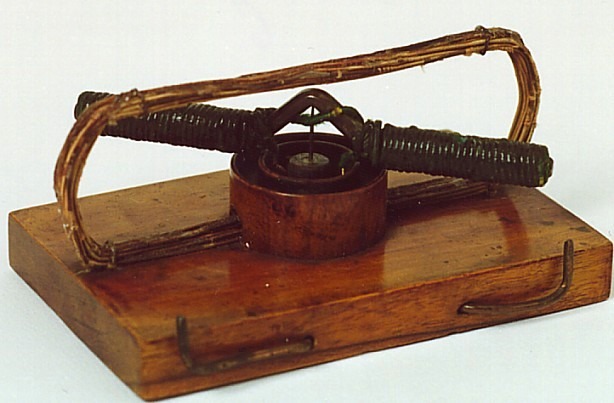
\includegraphics[width=\columnwidth]{Images/jedlik_motor.png} 
\caption[Jedlik's "Electromagnetic Self-Rotor"]{Jedlik's "Electromagnetic Self-Rotor". The historic motor created by the Hungarian physicist \'Anyos Jedlik still works perfectly today in the Museum of Applied Arts in Budapest.}
\label{fig:jedlik_motor}
\end{figure}

Due to the reduction of the prices of metals and the improvement and automation of manufacture processes, electric motors became available for a large range of applications, and not only as a research topic, up to the point that nowadays we interact with them in our daily life, sometimes without even noticing it. We have electric motors in all types of devices, from small applications like home appliances and hand-held gadgets, to large applications like robotics, cars and spaceships. As the complexity of the application increases, also the need for accuracy and efficiency does, leading to the development of more advanced electric motor technologies which lead to complex motion control techniques.

One of the most complex applications for motor control is robotics. The motion in a robotic system is part of its definition of automatic movement, therefore, a robotic system needs a predictable driving system to fulfil its purpose, which implies that most of the parameters of the motors inside the robot are known and that they can be controlled in a correct and precise way.

A challenging application regarding motors in robotics is the wheel driving, since it needs to be precise and powerful at the same time to transport the robotic system around large surfaces in an unmanned way, which means that there is no person on board and controlling the robot. For example, in robotic agriculture, which is one of the main reasons why this work was developed, a robot becomes an unmanned vehicle, which must transport itself around in farms, where the road represents harsh conditions for transportation, introducing the need for a precise drive to deal with small crops, a high torque to transport the robot in uneven grounds and a good range of speeds to displace itself in large field areas in the fastest way possible.

With aims to propose a solution for the land transportation in robotic agriculture projects, different types of motor technologies were studied a priori, finding out that in-wheel permanent-magnet brushless motors are one of the most suitable and currently used solutions to develop electric vehicles, since they don’t need an external system for power transmission from the motor to the wheels, taking advantage of the high stall torque property of the electric motors and the reduction of the space and weight that having a motor inside a wheel represents (\citeauthor{robi:2017}, \citeyear{robi:2017}).

To correctly drive permanent-magnet brushless motors, it is necessary to apply a proper driving technique, which becomes a complex task when the goal is to achieve the desired characteristics mentioned previously: a good precision, a high torque and a large range of speed. Given such a challenge, the development of electric motor drives becomes one of the topics that draws the interest of many engineers and scientists, also due to the multidisciplinary approach needed to reach the speed, torque and efficiency required to drive the development that the inventions of tomorrow require. The approach to improve the motor drive in the electronics engineering field is directly related to the development of the driving circuit topology and to the implementation of complex control algorithms in embedded software that improve the performance of the different motor technologies available.

Since the brushless motor technology is quite recent in comparison with the rest, there is still a lot of development going on regarding its driving, with aims to reach the highest efficiency possible at the lowest cost. The objective of this work was to develop an electronic driver to control brushless motors, taking as a study case the in-wheel motors that transport a skid-steering robot designed for robotic agriculture. We studied the available electronic architectures to design a motor driver, the different approaches to drive brushless motors, like the trapezoidal and the sinusoidal drive and the peripherals needed to make these driving happen. After studying these topics, the motor driver was physically implemented and tested, and from this, a new architecture was proposed from the results and conclusions obtained from the implementation and testing of the circuit.

\begin{figure}[htbp]
\centering
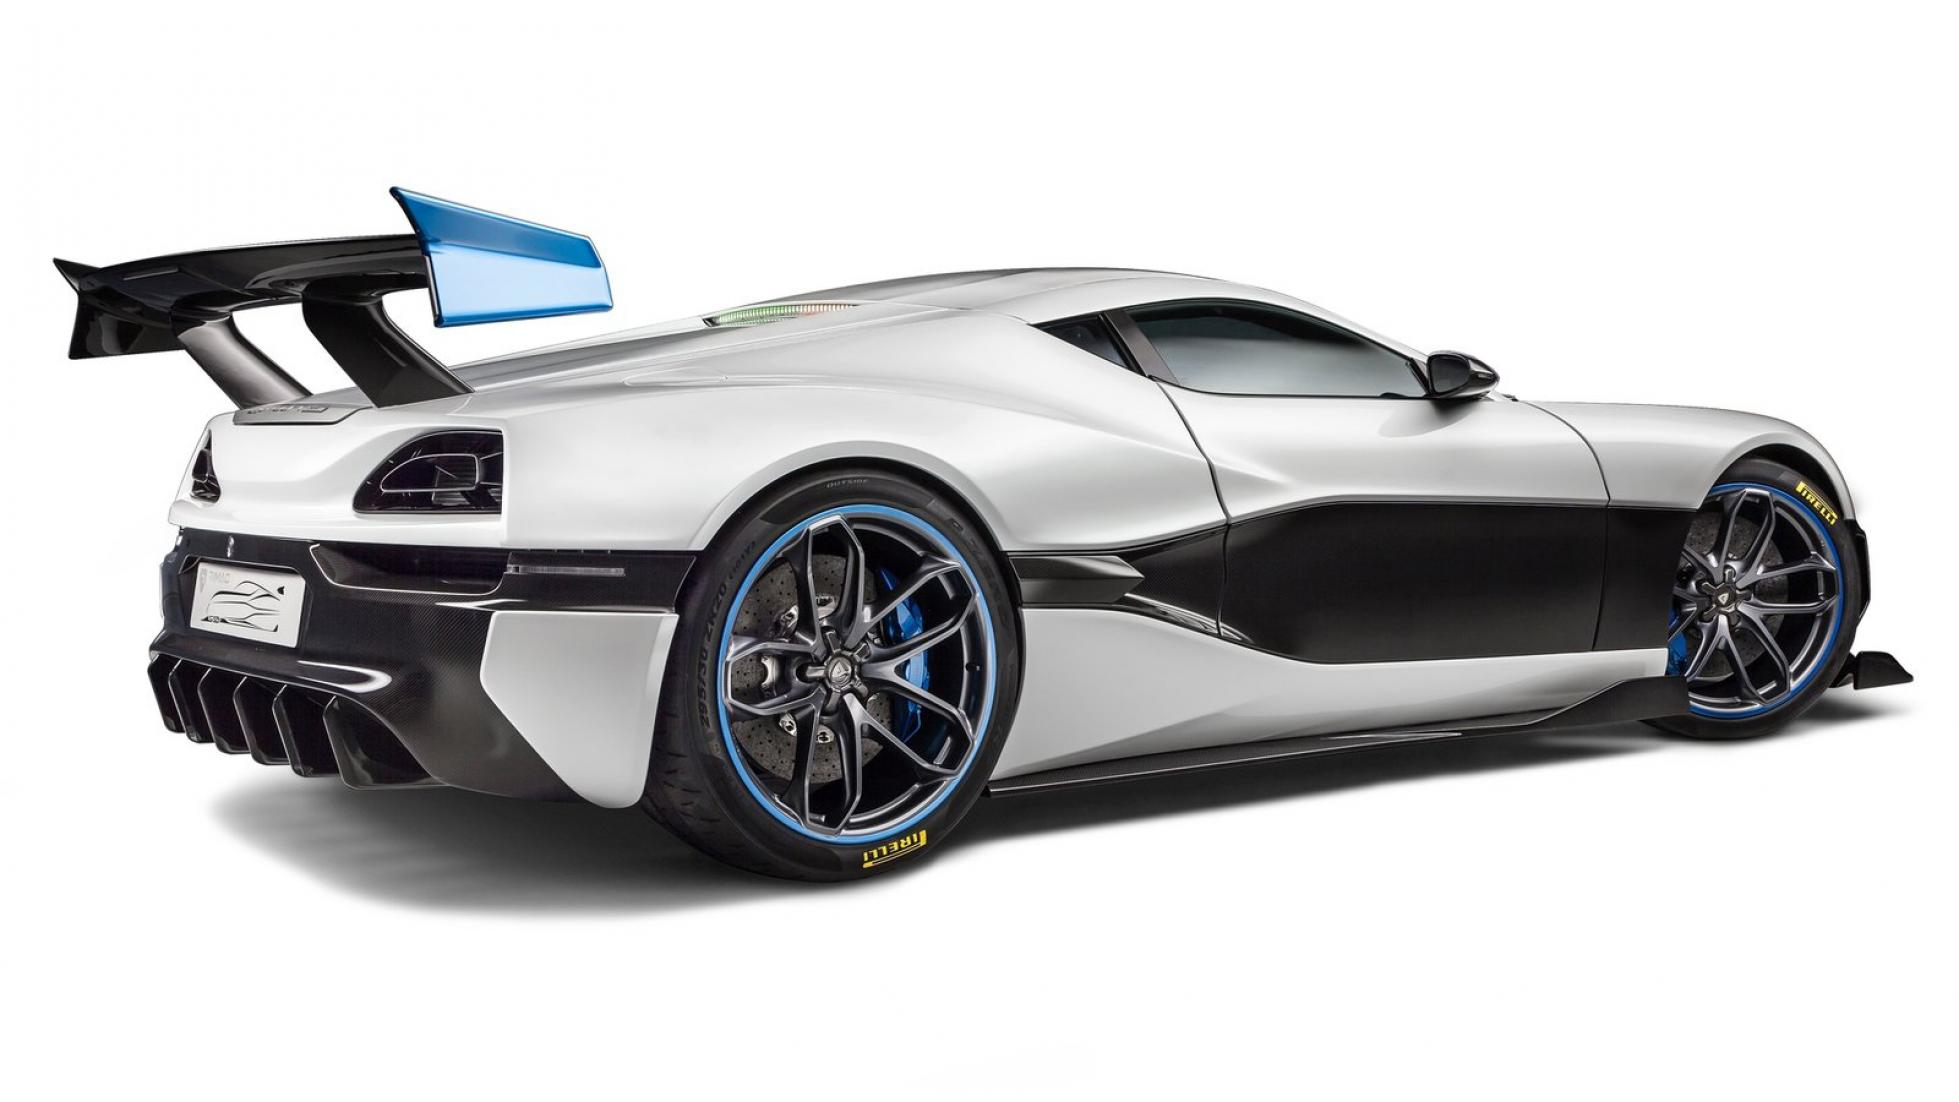
\includegraphics[width=\columnwidth]{Images/rimac-concept_s4.png} 
\caption[Rimac Concept S]{Rimac Automobili's electric supercar Concept S. Electric cars are becoming a trend and one of the main drivers for the development of technology related to electric motors.}
\label{fig:rimac_concept_s}
\end{figure}

This thesis explains in detail the most important information regarding the physical implementation of a motor driving system in such a way that it can be fully replicated. In Chapter \ref{chap:problem}, we explain more in detail the different reasons why this work was developed and the focus points that were stressed out. In Chapter \ref{chap:theory}, a simple but sufficient explanation about the theory behind the electric motor is given, explaining also the different existing technologies and their particular driving methods. In Chapter \ref{chap:robi} we explain the study case of ROBI', a prototype mobile manipulator for agricultural applications, which uses the in-wheel motor for which the motor driver of this work was developed. In Chapter \ref{chap:implementation} we explain in deep detail all the work developed around the implementation of the motor driver, both in the software and the hardware fields. In Chapter \ref{chap:results} we explain the final results of the work, showing and comparing graphs and waveforms of the behaviour of the in-wheel motor driven by the system developed. Finally, on Chapter \ref{chap:conclusion}, we discuss the results of the work realized and propose a new system, based on the implementation of the researched architecture and the problems encountered while working on the project.